%%%%%%%%%%%%%%%%%%%%%%%%%%%%%%%%%%%%%%%%%
% Tufte-Style Book (Documentation Template)
% LaTeX Template
% Version 1.0 (5/1/13)
%
% This template has been downloaded from:
% http://www.LaTeXTemplates.com
%
% Original author:
% The Tufte-LaTeX Developers (tufte-latex.googlecode.com)
%
% License:
% Apache License (Version 2.0)
%
% IMPORTANT NOTE:
% In addition to running BibTeX to compile the reference list from the .bib
% file, you will need to run MakeIndex to compile the index at the end of the
% document.
%
%%%%%%%%%%%%%%%%%%%%%%%%%%%%%%%%%%%%%%%%%

%----------------------------------------------------------------------------------------
%	PACKAGES AND OTHER DOCUMENT CONFIGURATIONS
%----------------------------------------------------------------------------------------

\documentclass{tufte-book} % Use the tufte-book class which in turn uses the tufte-common class

\hypersetup{colorlinks} % Comment this line if you don't wish to have colored links
\usepackage{amsmath}
\usepackage{amssymb}
\usepackage{amsthm}
\usepackage{listings}
\usepackage{siunitx} % align decimals in tables
\usepackage{nth}     % 1st, 2nd, ...
\usepackage{microtype} % Improves character and word spacing
\usepackage{asymptote} % for asymptote graphics
\usepackage{ccicons}
\usepackage{lipsum} % Inserts dummy text
\usepackage{booktabs} % Better horizontal rules in tables
\usepackage{graphicx} % Needed to insert images into the document
\theoremstyle{definition}
\newtheorem{definition}{Definition}
\theoremstyle{example}
\newtheorem{example}{Example}
\theoremstyle{theorem}
\newtheorem{theorem}{Theorem}
\graphicspath{{graphics/}} % Sets the default location of pictures

\setkeys{Gin}{width=\linewidth,totalheight=\textheight,keepaspectratio} % Improves figure scaling

\usepackage{fancyvrb} % Allows customization of verbatim environments
\fvset{fontsize=\normalsize} % The font size of all verbatim text can be changed here

\newcommand{\hangp}[1]{\makebox[0pt][r]{(}#1\makebox[0pt][l]{)}} % New command to create parentheses around text in tables which take up no horizontal space - this improves column spacing
\newcommand{\hangstar}{\makebox[0pt][l]{*}} % New command to create asterisks in tables which take up no horizontal space - this improves column spacing

\usepackage{xspace} % Used for printing a trailing space better than using a tilde (~) using the \xspace command

\newcommand{\Z}{\mathbb{Z}}
\newcommand{\R}{\mathbb{R}}
\newcommand{\andop}{\text{\ and\ }}
\newcommand{\orop}{\text{\ or\ }}
\DeclareMathOperator{\diag}{diag}
\DeclareMathOperator{\erf}{erf}
\DeclareMathOperator{\Prob}{Prob}
\DeclareMathOperator{\Var}{Var}


\newcommand{\monthyear}{\ifcase\month\or January\or February\or March\or April\or May\or June\or July\or August\or September\or October\or November\or December\fi\space\number\year} % A command to print the current month and year

\newcommand{\openepigraph}[2]{ % This block sets up a command for printing an epigraph with 2 arguments - the quote and the author
\begin{fullwidth}
\sffamily\large
\begin{doublespace}
\noindent\allcaps{#1}\\ % The quote
\noindent\allcaps{#2} % The author
\end{doublespace}
\end{fullwidth}
}

\newcommand{\blankpage}{\newpage\hbox{}\thispagestyle{empty}\newpage} % Command to insert a blank page

\usepackage{units} % Used for printing standard units

\newcommand{\hlred}[1]{\textcolor{Maroon}{#1}} % Print text in maroon
\newcommand{\hangleft}[1]{\makebox[0pt][r]{#1}} % Used for printing commands in the index, moves the slash left so the command name aligns with the rest of the text in the index 
\newcommand{\hairsp}{\hspace{1pt}} % Command to print a very short space
\newcommand{\ie}{\textit{i.\hairsp{}e.}\xspace} % Command to print i.e.
\newcommand{\eg}{\textit{e.\hairsp{}g.}\xspace} % Command to print e.g.
\newcommand{\na}{\quad--} % Used in tables for N/A cells
\newcommand{\measure}[3]{#1/#2$\times$\unit[#3]{pc}} % Typesets the font size, leading, and measure in the form of: 10/12x26 pc.
\newcommand{\tuftebs}{\symbol{'134}} % Command to print a backslash in tt type in OT1/T1

\providecommand{\XeLaTeX}{X\lower.5ex\hbox{\kern-0.15em\reflectbox{E}}\kern-0.1em\LaTeX}
\newcommand{\tXeLaTeX}{\XeLaTeX\index{XeLaTeX@\protect\XeLaTeX}} % Command to print the XeLaTeX logo while simultaneously adding the position to the index

\newcommand{\doccmdnoindex}[2][]{\texttt{\tuftebs#2}} % Command to print a command in texttt with a backslash of tt type without inserting the command into the index

\newcommand{\doccmddef}[2][]{\hlred{\texttt{\tuftebs#2}}\label{cmd:#2}\ifthenelse{\isempty{#1}} % Command to define a command in red and add it to the index
{ % If no package is specified, add the command to the index
\index{#2 command@\protect\hangleft{\texttt{\tuftebs}}\texttt{#2}}% Command name
}
{ % If a package is also specified as a second argument, add the command and package to the index
\index{#2 command@\protect\hangleft{\texttt{\tuftebs}}\texttt{#2} (\texttt{#1} package)}% Command name
\index{#1 package@\texttt{#1} package}\index{packages!#1@\texttt{#1}}% Package name
}}

\newcommand{\doccmd}[2][]{% Command to define a command and add it to the index
\texttt{\tuftebs#2}%
\ifthenelse{\isempty{#1}}% If no package is specified, add the command to the index
{%
\index{#2 command@\protect\hangleft{\texttt{\tuftebs}}\texttt{#2}}% Command name
}
{%
\index{#2 command@\protect\hangleft{\texttt{\tuftebs}}\texttt{#2} (\texttt{#1} package)}% Command name
\index{#1 package@\texttt{#1} package}\index{packages!#1@\texttt{#1}}% Package name
}}

% A bunch of new commands to print commands, arguments, environments, classes, etc within the text using the correct formatting
\newcommand{\docopt}[1]{\ensuremath{\langle}\textrm{\textit{#1}}\ensuremath{\rangle}}
\newcommand{\docarg}[1]{\textrm{\textit{#1}}}
\newenvironment{docspec}{\begin{quotation}\ttfamily\parskip0pt\parindent0pt\ignorespaces}{\end{quotation}}
\newcommand{\docenv}[1]{\texttt{#1}\index{#1 environment@\texttt{#1} environment}\index{environments!#1@\texttt{#1}}}
\newcommand{\docenvdef}[1]{\hlred{\texttt{#1}}\label{env:#1}\index{#1 environment@\texttt{#1} environment}\index{environments!#1@\texttt{#1}}}
\newcommand{\docpkg}[1]{\texttt{#1}\index{#1 package@\texttt{#1} package}\index{packages!#1@\texttt{#1}}}
\newcommand{\doccls}[1]{\texttt{#1}}
\newcommand{\docclsopt}[1]{\texttt{#1}\index{#1 class option@\texttt{#1} class option}\index{class options!#1@\texttt{#1}}}
\newcommand{\docclsoptdef}[1]{\hlred{\texttt{#1}}\label{clsopt:#1}\index{#1 class option@\texttt{#1} class option}\index{class options!#1@\texttt{#1}}}
\newcommand{\docmsg}[2]{\bigskip\begin{fullwidth}\noindent\ttfamily#1\end{fullwidth}\medskip\par\noindent#2}
\newcommand{\docfilehook}[2]{\texttt{#1}\index{file hooks!#2}\index{#1@\texttt{#1}}}
\newcommand{\doccounter}[1]{\texttt{#1}\index{#1 counter@\texttt{#1} counter}}

\usepackage{makeidx} % Used to generate the index
\makeindex % Generate the index which is printed at the end of the document

% This block contains a number of shortcuts used throughout the book

%----------------------------------------------------------------------------------------
%	BOOK META-INFORMATION
%----------------------------------------------------------------------------------------

\title{Luck} % Title of the book

\author[W. MacEvoy]{Warren D. MacEvoy} % Author

\publisher{Personal Notes} % Publisher

%----------------------------------------------------------------------------------------
\usepackage{ccicons}
\begin{document}

\def\asydir{graphics}
\begin{asydef}
// Global Asymptote definitions can be put here.
//import three;
//usepackage("bm");
//texpreamble("\def\V#1{\bm{#1}}");
// One can globally override the default toolbar settings here:
// settings.toolbar=true;
\end{asydef}
\frontmatter
\maketitle % Print the title page

%----------------------------------------------------------------------------------------
%	COPYRIGHT PAGE
%----------------------------------------------------------------------------------------

\newpage
\begin{fullwidth}
~\vfill
\thispagestyle{empty}
\setlength{\parindent}{0pt}
\setlength{\parskip}{\baselineskip}
Copyright \copyright\ \the\year\ \thanklessauthor

\par\smallcaps{Published by \thanklesspublisher}

\par\smallcaps{www.coloradomesa.edu}

\par \ccbyncsa\ [\url{http://creativecommons.org/licenses/by-nc-sa/4.0}]

You are free to:
\begin{itemize}
    \item Share -- copy and redistribute the material in any medium or format
    \item Adapt -- remix, transform, and build upon the material
\end{itemize}
Under the following terms:
\begin{itemize}
\item Attribution -- You must give appropriate credit, provide a link to the license, and indicate if changes were made. You may do so in any reasonable manner, but not in any way that suggests the licensor endorses you or your use.
\item NonCommercial -- You may not use the material for commercial purposes.
\item ShareAlike -- If you remix, transform, or build upon the material, you must distribute your contributions under the same license as the original. 
\end{itemize}\index{license}

\par\textit{First printing, \monthyear}
\end{fullwidth}

%----------------------------------------------------------------------------------------

\tableofcontents % Print the table of contents

%----------------------------------------------------------------------------------------

\listoffigures % Print a list of figures

%----------------------------------------------------------------------------------------

\listoftables % Print a list of tables

%----------------------------------------------------------------------------------------
%	DEDICATION PAGE
%----------------------------------------------------------------------------------------
%% \cleardoublepage
%% ~\vfill
%% \begin{doublespace}
%% \noindent\fontsize{18}{22}\selectfont\itshape
%% \nohyphenation
%% To Rose.
%% \end{doublespace}
%% \vfill
%% \vfill


\cleardoublepage
\chapter{Introduction}
\marginnote{This may exist as another name, but I don't think so, and it really should be called luck.  A Rose by the name of Rosaceae would be lost.}

The point of these notes is to introduce an idea of ``luck'' that connects mathematical probability with the everyday notion.

As a motivating problem, imagine walking along the beach and asking a random person to toss a tennis ball so that it lands in the sand.  The probability that it lands at some point would depend on the habits of the thrower and the details of the beach, but we can summarize this as some probability distribution, $p(x)=\rho(x) dx$, where $x\in\R^2$ is a suitable coordinate system for the beach in question.  It would almost certainly not be a uniform distribution, and it would almost certainly not be particularly concentrated.

Traditional probability feels uncomfortable here.  The chances of the ball landing at a given point is zero\marginnote{For a continuous probability distribution such as this, the chance of the ball landing in some small area $dx$ near $x$ is $p(x)=\rho(x) dx$.  But the ball lands at a point, so $dx$ is zero, so the probability $p(x)=\rho(x) dx$ is zero.}, and so miraculous.  Yet anyone watching this process would only occasionally be surprised by the outcome.

As common (and mundane, not miraculous) such situations are, the language of statistics seems to have difficulty with the notion.  Nor is it limited to continuous cases, just when there are a lot of possible outcomes.  Such examples lead to non-zero but very small probabilities.\marginnote{The real motivation of this came from the space of passwords a person might choose from, which is an effectively infinite discrete space.}

To distinguish from the more general notion of luck, note that that there is no extrinsic value on an outcome.  To say something is ``lucky'' often means there is some value (different from the probability) associated with outcomes.  However, outcomes that are the most valuable are often the least probable, and outcomes of equal probability ought to be equally lucky.  In the most extreme case of all equally probable outcomes (uniform probability), every outcome should have a luck of $\frac{1}{2}$.  

These observations lead to the following definition of luck:
\begin{quote}
\index{luck $L$ ! informal}
The luck $L(x)$ of an outcome $x$ is the probability of getting any outcome $y$ that is more probable than $x$, plus one-half the probability of getting any outcome $y$ that is equally probable to $x$.
\end{quote}

From the perspective of discussing luck, it is convenient to have few sets: $\Omega(x)$, the outcomes more likely than $x$, and $\omega(x)$, the outcomes equally likely to $x$.

\begin{definition}{Omega.}  $\Omega(x)$ is set of outcomes more likely than $x$:
\begin{equation}
\index{Omega $\Omega$ ! definition}
\Omega(x) = \left\{ y \mid p(y)>p(x) \right\} \,.
\end{equation}
We define $|\Omega(x)|$ as the probability an outcome is in $\Omega(x)$,
$|\Omega(x)| = P(y\in\Omega(x))$.  In the discrete case, this is
\begin{equation}
\index{Omega $\Omega$ ! size $\abs{\Omega}$ (discrete)}
|\Omega(x)| = \sum_{y \in \Omega(x)} p(y),
\end{equation}
and, in the continuous case,
\begin{equation}
\index{Omega $\Omega$ ! size $\abs{\Omega}$ (continuous)}
|\Omega(x)| = \int_{\Omega(x)} \rho(y)\,dy \,.
\end{equation}
\end{definition}

\begin{definition}{omega.}\marginnote{For the typical case of many outcomes with different probabilities, $|\omega(x)|$ is small.  For example, $|\omega(x)|=0$ for any multivariate normal distribution.}
$\omega(x)$ is the set of outcomes equally likley to $x$:
\begin{equation}
\index{omega $\omega$ ! definition}
\omega(x) = \left\{ y \mid p(y)=p(x) \right\} \,.
\end{equation}
Similar to $\Omega(x)$, we define $|\omega(x)|$ as the probability an outcome is in $\omega(x)$,
$|\omega(x)| = P(y\in\omega(x))$.  

In the discrete case, this is
\begin{equation}
\index{omega $\omega$ ! size $\abs{\omega}$ (discrete)}
|\omega(x)| = \sum_{y \in \omega(x)} p(y),
\end{equation}
and, in the continuous case,
\begin{equation}
\index{omega $\omega$ ! size $\abs{\omega}$ (continuous)}
|\omega(x)| = \int_{\omega(x)} \rho(y)\,dy \,.
\end{equation}
\end{definition}

With these definitions in place, we define luck mathematically as follows:
\begin{definition}{Luck.}  The luck of an outcome is the probability getting any more likely outcome, plus half the probability of getting any equally likely outcome:
\begin{equation}
\index{luck $L$ ! definition}
L(x)=|\Omega(x)| + \frac{1}{2} |\omega(x)| \,.
\end{equation}
\end{definition}

\subsection{Properties of Luck.}
\index{luck $L$ ! properties}
\begin{itemize}
\item Range of luck. $0 \leq L(x) \leq 1$.  This ranges from no luck to perfect luck.
\item Lucky outcomes. If $L(x)$ is close to 1, then $p(x)$ is comparatively small, and most outcomes would have a higher probability (you are lucky).  
\item Unlucky outcomes. If $L(x)$ is close to 0, then $p(x)$ is comparatively large, and most outcomes would have a lower probability (you are unlucky).
\item Luck on average. $E(L)=\frac{1}{2}$.  On average, luck is always 50:50.
\end{itemize}

We are interested in cases which have many possible outcomes with low but somewhat different probabilities (like the tennis ball on the beach).  If the space is well divided (so $\max |\omega|=\max_{x}|\omega(x)|$ is small), then there are other interesting properties of luck:\marginnote{In particular $|\omega(x)|=0$ for the normal, exponential, beta, and gamma distributions.  As a worst-case counterexample, the flattest distribution is the uniform distribution, for which $|\omega(x)|=1$.}

For the kind of distributions with small $\max |\omega|$, luck is a very uniformizing transformation (there can be no better, actually).  If it were exactly uniform, the following would be correct with $\varepsilon=0$.  There is no other functional of the probability space alone with smaller error bounds:
\begin{itemize}
\index{luck $L$ ! uniformity}
\item For any $f: [0,1] \rightarrow \mathbb{R}$ with bounded second derivative, $E(f(L))=\int_0^1 f(L) dL-\varepsilon$, where $|\varepsilon| \leq \max|f''| \cdot \max |\omega|^2 / 24$.
\item For $p \geq 2$, $E(L^p)=1/(p+1)-\varepsilon$, $0 \leq \varepsilon \leq p \cdot (p-1) \max |\omega|^2/24$.
\item For $0 \leq a \leq b \leq 1$, $E(L \in [a,b])=b-a - \varepsilon$, $|\varepsilon| \leq \max |\omega|$.
\end{itemize}
The proofs of these come from the midpoint integration rule and thinking about the general case for figure~\ref{fig:arrange} below.

\begin{example}{Eight Fair Coins.}
\index{examples ! eight fair coins}
Suppose we toss 8 fair coins.  The probability of getting exactly $x$ heads out of 8 tosses is given by the binomial distribution
\begin{equation}
p(x)=\frac{8!}{x!(8-x)!}\left(\frac{1}{2}\right)^8 \,.
\end{equation}
What is the luck associated with this distribution?
\begin{table}
\caption{This is arranged in increasing luck (which is decreasing probability). Getting exactly $x=4$ heads is unlucky, requiring only $L=14\%$ luck, while getting $x=0$ or $x=8$ heads is almost $100\%$ luck.}
\begin{tabular}{|c|S[table-format=2.4]|c|S[table-format=2.4]|c|S[table-format=2.4]|c|S[table-format=2.4]|S[table-format=2.4]|}
\multicolumn{1}{c}{$x$} &
\multicolumn{1}{c}{$p(x)$} &
\multicolumn{1}{c}{$\Omega(x)$} &
\multicolumn{1}{c}{$|\Omega(x)|$} &
\multicolumn{1}{c}{$\omega(x)$} &
\multicolumn{1}{c}{$|\omega(x)|$} &
\multicolumn{1}{c}{$L(x)$} \\
\hline
     4 & 0.2734 &  \{\} & 0.0000 & \{4\} & 0.2734 & 0.1367 \\
3 or 5 & 0.2188 & \{4\} & 0.2734 & \{3,5\} & 0.4375 & 0.4922 \\
2 or 6 & 0.1094 & \{3,4,5\} & 0.7109 & \{2,6\} & 0.2188 & 0.8203 \\
1 or 7 & 0.0313 & \{2,3,4,5,6\} & 0.9297 & \{1,7\} & 0.0625 & 0.9609 \\
0 or 8 & 0.0039 & \{1,2,3,4,5,6,7\} & 0.9922 & \{0,8\} & 0.0078 & 0.9961 \\
\hline
\end{tabular}
\end{table}
\begin{figure}
\begin{center}
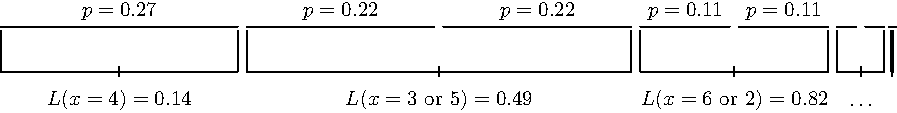
\includegraphics[width=1.00\linewidth]{graphics/arrange.pdf}
\end{center}
\caption{\label{fig:arrange}Luck to get $x$ heads on $8$ fair coins.  After the probabilities are arranged in decreasing order on the unit interval, $L(x)$ is the center point of equally probable outcomes.}
\label{fig:arrange}
\end{figure}

Luck on average is $\frac{1}{2}$:
\marginnote{For any distribution, $E(L)=\frac{1}{2}$.}
\begin{equation}
E(L)=\sum_{x=0}^8 p(x) \cdot L(x) = \frac{1}{2} \,.
\end{equation}

The second moment should be close to $\frac{1}{3}$:
\marginnote{For any distribution, $E(L^2)=\frac{1}{3}-\varepsilon$, with $0 \leq \varepsilon \leq \max |\omega|^2/12$.

For the coin distribution, the bound is $0 \leq \varepsilon \leq 0.016$, and the actual error $\varepsilon=0.0096$.}
\begin{equation}
E(L^2)=\sum_{x=0}^8 p(x) \cdot L(x)^2 = \frac{1}{3} - 0.0096
\end{equation}

The probability luck is in the middle half is about $\frac{1}{2}$:
\marginnote{For any distribution, $E(L \in [a,b]) = b-a+\varepsilon$, with $|\varepsilon|\leq \max |\omega|$.

For the coin distribution and $[a,b]=[\frac{1}{4},\frac{3}{4}]$, $E(L \in [a,b])=\frac{1}{2}+\varepsilon$ with $|\varepsilon|\leq 0.4375$ as the (poor) error bound, and the actual error of $\varepsilon=-0.0625$}
\begin{equation}
\begin{split}
E(L \in [\frac{1}{4},\frac{3}{4}]) &= \sum_{x=0}^8 p(x) \cdot 
\left\{ \begin{array}{cl} 1 & \text{if $L(x) \in [\frac{1}{4},\frac{3}{4}]$} \\
                          0 & \text{otherwise} 
\end{array} \right\} \\
&= \frac{1}{2} - 0.0625 \,.
\end{split}
\end{equation}
\end{example}
\begin{example}{Normal ($d_f=1$).}
\index{examples ! normal ($d_f=1$)}
This is a special case of the multivariate normal we cover in the next section, but working out the details for the one-dimensional case can be illuminating.  We define the one-dimensional normal distribution with mean $\mu$ and variance $\Sigma$ as
\begin{align}
P_{\text{normal}}(x;\mu,\Sigma) &= \frac{e^{-\frac{(x-\mu)^2}{2\Sigma}}}{\sqrt{2\pi\Sigma}} \,,\\
\intertext{where}
\mu &= E(x)\,,\\
\intertext{and}
\Sigma &= E((x-\mu)^2) \,.
\end{align}

First note that $\Omega(x)$ is the open the interval between $x$ and $x$ reflected around $\mu$:
\begin{equation}
\Omega(x)=(\min(x,2\mu-x),\max(x,2\mu-x)) \,,
\end{equation}
and $\omega(x)$ is the endpoints of that interval:
\begin{equation}
\omega(x)=\{x,2\mu-x\} \,.
\end{equation}

Since the 1-dimensional normal distribution is a continuous distribution and $\omega(x)$ is a finite set, $|\omega(x)|=0$, i.e.,
\begin{equation}
|\omega(x)|=\int_{\omega(x)} P_{\text{normal}}(y;\mu,\Sigma) \, dy = 0 \,.
\end{equation}
This means all the luck properties are exact (the error terms are zero), and the $\frac{1}{2}|\omega(x)|$ contributes nothing to the luck of an outcome.

What remains is to calculate luck,
\begin{equation}
L(x)=\int_{\Omega(x)} P_{\text{normal}}(y;\mu,\Sigma) \, dy \,.
\end{equation}
Changing variables to the normalized $z$-score: $z=\sqrt{\Sigma^{-1}}(x-\mu)$, this can be rewritten as
\begin{equation}
L(x)=\int_{-R}^{R} P_{\text{normal}}(y,0,1) \, dy \,,
\end{equation}
where
\begin{equation}
R=|\sqrt{\Sigma^{-1}}(x-\mu)| \,.
\end{equation}

Using $\erf(x)$, defined as\marginnote{$\erf(x)$ is a normalized integral of the $P_{\text{normal}}(x;\mu=0,\Sigma=1/2)$ so that $\erf(0)=0$ and $\erf(\pm \infty)=\pm 1$.}
\begin{equation}
\erf(x) = \frac{2}{\sqrt{\pi}} \int_0^x e^{-y^2} \, dy \,, 
\end{equation}
the luck of an outcome can be written as
\begin{equation}
\label{eq:normal-1d-luck}
L(x)=\erf\left|\frac{x-\mu}{\sqrt{2\Sigma}} \right| \,.
\end{equation}

In the next chapter, where we address the more general multivariate normal case, we obtain the approximation,
\begin{equation}
\label{eq:approx-normal-1d-luck}
L(x) \approx \frac{1}{2} \left[ 1+\erf\left(\left|\frac{x-\mu}{\sqrt{\Sigma}} \right|-\sqrt{\frac{1}{2}}\right)\right] \,.
\end{equation}
Figure~\ref{fig:normal1} compares the exact and approximate result in the 1-d case.

\begin{figure}
\begin{center}
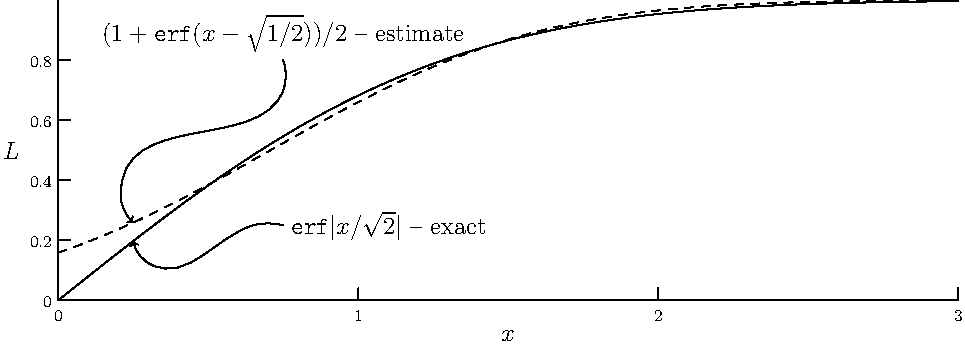
\includegraphics[width=0.75\linewidth]{graphics/normal1.pdf}
\end{center}
\caption{Exact (solid, equation~\ref{eq:normal-1d-luck}) vs approximate (dashed, equation~\ref{eq:approx-normal-1d-luck}) luck for 1-d normal distribution.}
\label{fig:normal1}
\end{figure}
\end{example}

\begin{example}{$\rchi^2$ $p$-value vs. $L$}
\index{examples ! $\rchi^2$ $p$-value vs. $L$}

For symmetric or monotonic one dimensional continuous distributions, the connection between luck and $p$-values can be pretty simple.  However, the relation between $p$ and $L$ can be complex.  Figure~\ref{fig:chi2} shows the $p$-values vs luck for $\rchi^2_k(x)$ for $k=4$ distribution.

\begin{figure}
\begin{center}
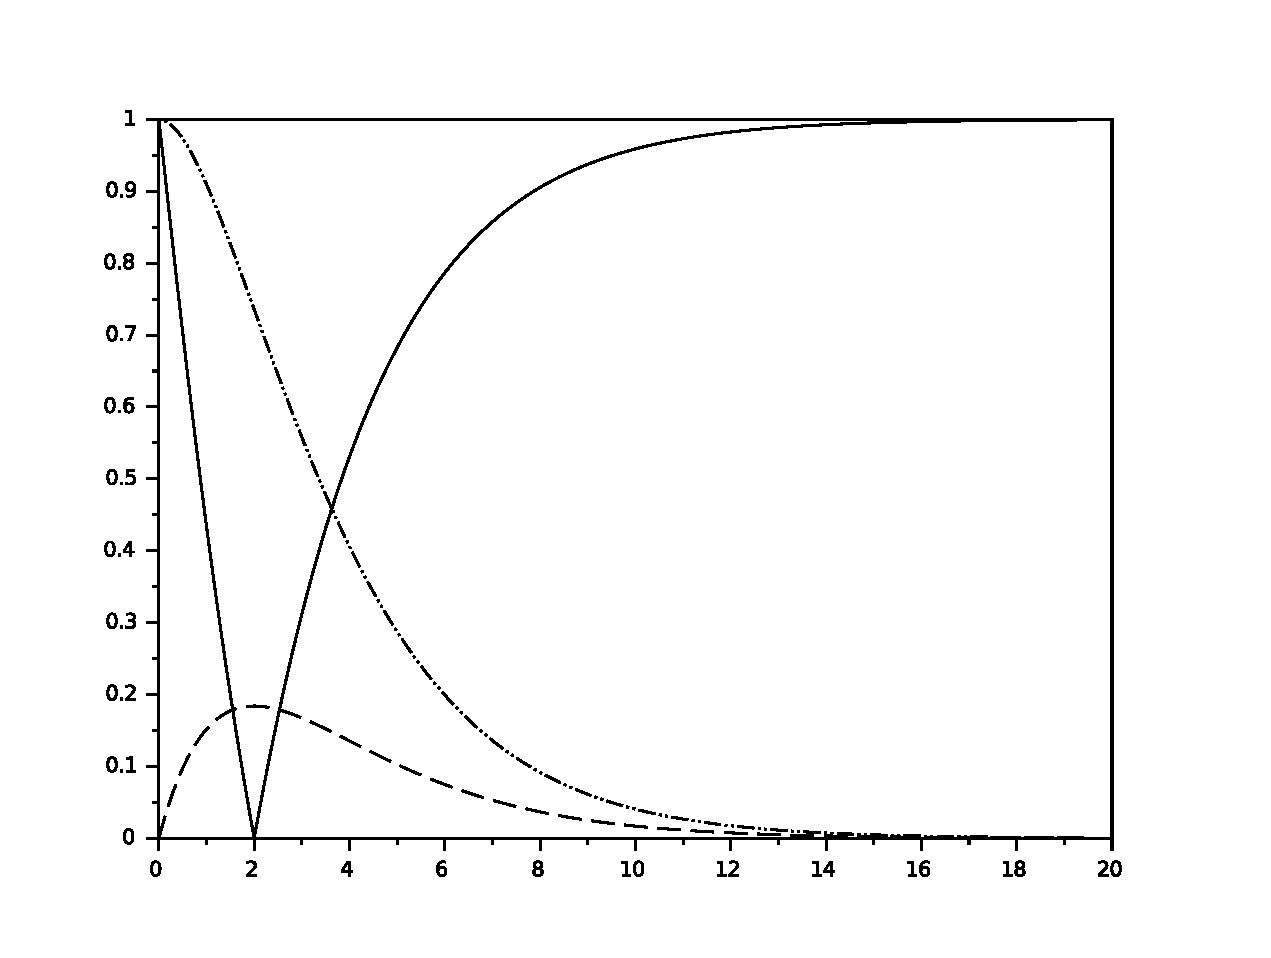
\includegraphics[width=0.75\linewidth]{img/chi2.pdf}
\end{center}
\caption{$p$-value (dotted) vs $L$ (solid) for the $\rchi^2$ distribution for $k=4$ (dashed).  There is no simple relationship between $L$ and $p$.}
\label{fig:chi2}
\end{figure}
In the chapter on $\rchi^2$, we show a good approximation for large $k$ is
\begin{equation}
  L[\rchi^2_k](x)\approx \erf \left|\sqrt{x}-\sqrt{k-2}\right| \,.
\end{equation}
\end{example}

\section{Summary}
\begin{itemize}
\item Luck has a natural definition of
  \begin{equation*}
    \begin{split}
    \Luck(x) = &\Prob(\text{anything more likely than $x$}) \\
    & + \frac{1}{2} \Prob(\text{$x$ or anything equally likely to $x$}) \,.
    \end{split}
    \end{equation*}
  \item Luck ranges from $0$ (no luck) to $1$ (perfect luck).
  \item The expected value of luck is always exactly $1/2$.
  \item Luck is very nearly uniform, and there is no better map to a uniform distribution for a general probability distribution. 
  \item For the $d_f=1$ normal distribution with mean $\mu$ and standard deviation $\sigma$:
    \begin{equation*}
L[{\cal N}_{1d}(\cdot;\mu,\sigma^2)](x)=\erf \left|\frac{x-\mu}{\sqrt{2} \sigma} \right| \,.      
    \end{equation*}
  \item For the $\rchi^2_k$ distribution, there is no simple form, but for large $k$:
    \begin{equation*}
      L[\rchi^2_k](x) \approx \erf \left| \sqrt{x}-\sqrt{k-2} \right| \,.
    \end{equation*}
\end{itemize}

\section{Exercises}
\begin{enumerate}
\item \label{q:intro-coin} Take the maximum of two fair coin flips (0 or 1), so $\Prob(\max = 0)=1/4$ and $\Prob(\max = 1)=3/4$.  What is the luck of each outcome?
\item \label{q:intro-coins} Take 3 independent trials like problem \ref{q:intro-coin}.  Note there are $2^3$ outcomes but only 4 distinct probabilities.  Show that
  \begin{gather*}
    L((1,1,1))=\frac{27}{128} \approx 0.2109 \\
    L((0,1,1))=L((1,0,1))=L((1,1,0))=\frac{81}{128} \approx 0.6328 \\
    L((1,0,0))=L((0,1,0))=L((0,0,1))=\frac{117}{128} \approx 0.9141 \\
    L((0,0,0))=\frac{127}{128} \approx 0.9922
  \end{gather*}
\item \label{q:intro-coin-test} Use a strong random number generator (like {\tt random.org}) to make 3 independent trials for the maximum of 2 fair coin tosses.  What is the luck of the outcome?
\item \label{q:intro-exp} Now write down what feels like a random sequence of six zeros and ones --- don't think too hard about it!  Use these in pairs like problem \ref{q:intro-coin-test}.  What was the luck of this outcome?
\item Calculate the luck $L(x)$ for the exponential distribution $p(x)=\lambda \exp(-\lambda x)$ for $x\geq 0$ and $\lambda > 0$.

\item In {\em Rosencrantz and Guildenstern Are Dead}, Guildenstern tosses 85 heads in a row at the beginning of the play.  Taken as a sequence of fair coin tosses, why is Guildenstern luck 1/2?

\item Ignoring the last coin toss, group the 84 heads as 42 experiment pairs like problem \ref{q:intro-coin}.  Show from this perspective Guildenstern is unlucky:
  \begin{equation*}
    L=\frac{109418989131512359209}{38685626227668133590597632} \approx 2.828 \times 10^{-6} \,.
  \end{equation*}
\item Now consider the minimum-of-pairs problem for the 42 head-pairs.  Show that for this problem Guildenstern is insanely lucky:
  \begin{equation*}  
  L=1-2^{-85} \approx 1-2.585\times 10^{-26}
  \end{equation*}
\end{enumerate}


\chapter{Normal Distribution}
Suppose we are in a probability space well approximated by the multivariate normal (Gaussian) distribution of a random variable $x \in \R^n$ with mean $\mu$ and non-singular covariance $\Sigma$:
\marginnote{The $n=1$ example in the introduction is just where where $\mu$ and $\Sigma$ are scalars.}
\begin{align}
P_{\text{normal}}(x;\mu,\Sigma) &= \frac{e^{-\frac{1}{2}(x-\mu)^T \Sigma^{-1} (x-\mu)}}{\sqrt{(2\pi)^n \det{\Sigma}}}  \,,\\
\intertext{where}
\mu_i &= E(x_i)\,,\\
\intertext{and}
\Sigma_{ij} &= E((x_i-\mu_i)(x_j-\mu_j)) \,.
\end{align}

How lucky is some outcome $x$? From the definition:
\begin{align}
L(x)&=|\Omega(x)|+\frac{1}{2}|\omega(x)| \,,\\
\intertext{where}
\Omega(x) =& \left\{ y \in \R^n \middle| P_{\text{normal}}(y) > P_{\text{normal}}(x) \right\} \\
          =& \left\{ y \in \R^n \middle| |\sqrt{\Sigma^{-1}}(y-\mu)| < |\sqrt{\Sigma^{-1}}(x-\mu)| \right\}
\intertext{and}
\omega(x) =& \left\{ y \in \R^n \middle| |\sqrt{\Sigma^{-1}}(y-\mu)| = |\sqrt{\Sigma^{-1}}(x-\mu)| \right\} \,.
\end{align}
Because $\omega(x)$ has no volume in $\R^n$,
\begin{equation}
|\omega(x)|=\int_{\omega(x)} P_{\text{normal}}(y;\mu,\Sigma) \, dy = 0 \,.
\end{equation}

 So
\begin{align}
L(x) &=|\Omega(x)|\\
     &=\int_{\Omega(x)} P_{\text{normal}}(y;\mu,\Sigma) \,dy\,.
\end{align}

\marginnote{$\Sigma$ is symmetric and positive definite, and so is its inverse.  The square-root can be computed as a Cholesky decomposition.  In Scilab, \lstinline[language=Scilab]{z=chol(Sigma)'\\(x-mu)}}
By changing variables to $z=\sqrt{\Sigma^{-1}} (x-\mu)$,
\begin{equation}
L(x) = \int_{|z|<R}  P_{\text{normal}}(z;0,I) \, dz \,,
\end{equation}
\marginnote{\lstinline[language=Scilab]{R=norm(z)}}
where $R = |\sqrt{\Sigma^{-1}} (x-\mu)|$.

This can be evaluated in spherical coordinates:
\begin{align}
\label{eq:normal-luck-as-integral}
L(x)    &=\frac{1}{\sqrt{(2\pi)^{n}}} \int_{0}^{R} \frac{n \pi^{n/2}}{\Gamma(\frac{n}{2}+1)} r^{n-1} e^{-\frac{1}{2} r^2} \, dr \,, \\
    &=\frac{\gamma(n/2,R^2/2)}{\Gamma(n/2)} \,.
\end{align}
\marginnote{\lstinline[language=Scilab]{L=cdfgam("PQ",R^2/2,n/2,1)}}
The last form uses the lower incomplete gamma function and gamma function, defined to be
\begin{align}
\gamma(s,x) &= \int_0^{x} t^{s-1} e^{-t} \, dt \\
\Gamma(s) &= \gamma(s,\infty) \,.
\end{align}
For any value of $n$, but particularly for large values, we find the following approximation to be very good\marginnote{This comes from a Taylor expansion of the log of the integrand in (\ref{eq:normal-luck-as-integral}), which is specifically invalid for $n=1$, hence the difference between the general case and the $n=1$ case (\ref{eq:normal-1d-luck}).}:
\marginnote{\lstinline[language=Scilab]{Lapprox=0.5*(1+erf(R-sqrt(n-1/2)))}}
\begin{equation}
\label{eq:normal-luck-approx}
L(x) \approx \frac{1}{2}\left[1+\erf(|\sqrt{\Sigma^{-1}} (x-\mu)|-\sqrt{n-1/2})\right] \,.
\end{equation}
\begin{figure}
  \caption{Exact (blue) vs approximate (red) luck for normal distribution for $n=1$, $10$, and $100$.}
  \centering
    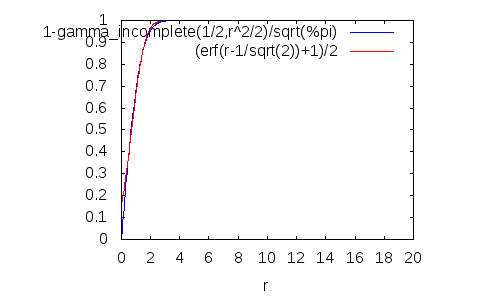
\includegraphics[width=0.75\textwidth]{img/luck1}
    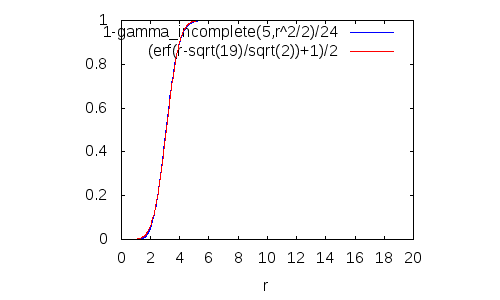
\includegraphics[width=0.75\textwidth]{img/luck10}
    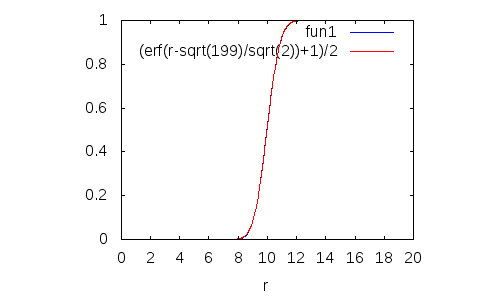
\includegraphics[width=0.75\textwidth]{img/luck100}
\end{figure}

Not only is this result pretty, it is very useful.  Suppose we have distribution parameters $\mu$ and $\Sigma$, and would like to know if they fit actual observations.  A traditional approach requires a large sample to estimate $\mu$ and $\Sigma$, but we don't need this, nor do we need to assume that the distribution is normal.  We just need to ask if the observations are surprising (lucky or unlucky).  In large dimensions, numerical experiments suggest one sample is in most cases sufficient to establish practical certainty (probability of error less than $10^{-15}$).
\begin{table}
\caption{\label{tab:normal}Luck from two randomly generated distributions $\mu^{(x)}$ and $\mu^{(y)}$ uniformly chosen in $[0,1]^{100}$, and $\Sigma^{(x)}, \Sigma^{(y)}$ are transposed squares of random $100 \times 100$ matrices.  In each row, $x$ is  a sample from the $\mu^{(x)},\Sigma^{(x)}$, normal distribution, and $y$ is from the $\mu^{(y)},\Sigma^{(y)}$ distribution.  The actual values of $x$ and $y$ are not given, since they are very large (100 numbers each) and uninteresting.}
\begin{tabular}{|S[table-format=2.10]|S[table-format=2.10]|S[table-format=2.10]|S[table-format=2.10]|}
\multicolumn{1}{c}{$L^{(x)}(x)$} &
\multicolumn{1}{c}{$L^{(y)}(x)$} &
\multicolumn{1}{c}{$L^{(x)}(y)$} &
\multicolumn{1}{c}{$L^{(y)}(y)$} \\
\hline
0.5014172020 & 1.0000000000 & 1.0000000000 & 0.8381802641 \\
0.7314212665 & 1.0000000000 & 1.0000000000 & 0.2392581432 \\
0.9825630339 & 1.0000000000 & 1.0000000000 & 0.2716955127 \\
0.0334550807 & 1.0000000000 & 1.0000000000 & 0.4213206259 \\
0.6894299340 & 1.0000000000 & 1.0000000000 & 0.0744616557 \\
0.7363975937 & 1.0000000000 & 1.0000000000 & 0.2940507284 \\
0.3045212967 & 1.0000000000 & 1.0000000000 & 0.7078490147 \\
0.2311115744 & 1.0000000000 & 1.0000000000 & 0.2903130932 \\
0.5852477199 & 1.0000000000 & 1.0000000000 & 0.6369022028 \\
0.2145529261 & 1.0000000000 & 1.0000000000 & 0.2689897874
\end{tabular}
\end{table}

\subsection{Combining Normal Luck}
The approximate result (\ref{eq:normal-luck-approx}) leads to a rule for combining (normal) luck:  Suppose there are two independent normal distributions parameterized by $\mu^{(x)}$ , $\Sigma^{(x)}$ of dimension $n_x$, and $\mu^{(y)}$, $\Sigma^{(y)}$ of dimension $n_y$.  What is the luck of a single combined observation $(x,y)$?
\begin{align}
L(x,y) &\approx \frac{1}{2}\left[1+\erf(\sqrt{R_x(x)^2+R_y(y)^2}-\sqrt{n_x+n_y-\frac{1}{2}}) \right] \,,
\intertext{where}
R_x(x) &= \erf^{-1}(2L_x -1)-\sqrt{n_x-\frac{1}{2}} = \sqrt{\left(\Sigma^{(x)}\right)^{-1}} \left(x-\mu^{(x)}\right) \,, \\
R_y(y) &= \erf^{-1}(2L_y -1)-\sqrt{n_y-\frac{1}{2}} = \sqrt{\left(\Sigma^{(y)}\right)^{-1}} \left(y-\mu^{(y)}\right) \,.
\end{align}

\begin{figure}
  \caption{Histograms of 10,000 luck values in the same distributions as table~\ref{tab:normal}.  Upshot: $y$ values in the $x$ distribution are viewed as extremely lucky and vice-versa, while they are have uniform luck in their own respective distributions.}
  \centering
    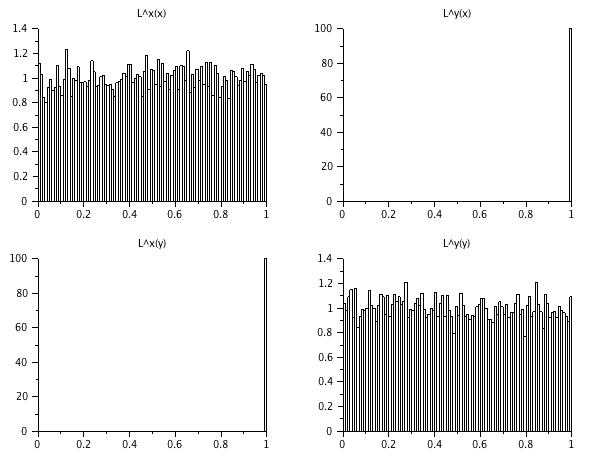
\includegraphics[width=0.75\textwidth]{img/normal}
\end{figure}

The listings in figures \ref{fig:mnprobln}-\ref{fig:mnapproxluck} give Scilab functions for basic luck calculations for multivariate normal distributions.

\begin{figure}
\caption{\label{fig:mnprobln}Scilab listing to compute the natural log of the probability of multivariate normal outcomes.  $x$ is a $n_{\text{dim}} \times n_{\text{samps}}$ of outcomes, $\mu$ is a $n_{\text{dim}} \times 1$ column vector of the means, and $\Sigma$ is a $n_{\text{dim}} \times n_{\text{dim}}$ covariance matrix.  The result {\tt lnp} is a $1 \times n_{\text{samps}}$ row vector.}
\lstset{language=Scilab}
\begin{lstlisting}
function lnp=mnprobln(x,mu,Sigma)
  [dim,nsamps]=size(x);
  sigma=chol(Sigma)';
  z=sigma\(x-mu*ones(1,nsamps));
  R2=sum(z.^2,'r');
  lnp=-R2/2-(dim/2*log(2*%pi)+...
       sum(log(diag(sigma))));
endfunction
\end{lstlisting}
\end{figure}

\begin{figure}
\caption{\label{fig:mnluck}Scilab listing to efficiently compute the luck of multivariate normal outcomes.  $x$ is a $n_{\text{dim}} \times n_{\text{samps}}$ of outcomes, $\mu$ is a $n_{\text{dim}} \times 1$ column vector of the means, and $\Sigma$ is a $n_{\text{dim}} \times n_{\text{dim}}$ covariance matrix.  The result $L$ is a $1 \times n_{\text{samps}}$ row vector of the luck associated with each outcome.}
\lstset{language=Scilab}
\begin{lstlisting}
function L=mnluck(x,mu,Sigma)
  [dim,nsamps]=size(x);
  one=ones(1,nsamps);
  sigma=chol(Sigma)';
  z=sigma\(x-mu*one);
  R2=sum(z.^2,'r');
  L=cdfgam("PQ",R2/2,dim/2*one,one);
endfunction
\end{lstlisting}
\end{figure}

\begin{figure}
\caption{\label{fig:mnapproxluck}Like {\tt mnluck} in figure~\ref{fig:mnluck}, but approximates luck via (\ref{eq:normal-luck-approx}).}
\lstset{language=Scilab}
\begin{lstlisting}
function L=mnapproxluck(x,mu,Sigma)
  [dim,nsamps]=size(x);
  sigma=chol(Sigma)';
  z=sigma\(x-mu*ones(1,nsamps));
  R=sqrt(sum(z.^2,'r'));
  L=0.5*(1+erf(R-sqrt(dim-0.5)));
endfunction
\end{lstlisting}
\end{figure}

\chapter{Multinomial Distribution}
Selecting independent samples (with repetition) from a discrete set of outcomes follows the multinomial distribution.

Specifically, select $N$ independent samples (with repetition) from a discrete set of possible outcomes $\left\{x_i \in \Z_{0+}\right\}_{i=1}^{n}$ with probabilities $p_i$,  $\sum_{i=1}^{n} p_i = 1$.  Not considering order, this will result in $x_i \in Z_{0+}$ counts of outcome $w_i$, $\sum_{i=1}^{N_P} x_i = N$.
The probability of such a sample is given by the multinomial distribution:
\begin{equation}
\index{multinomial ! probability}
\label{eq:multinomial}
P_{\text{multinomial}}(x;p)={N!}\prod_{i=1}^{n} \frac{p_i^{x_i}}{x_i!} \,. 
\end{equation}

The counts $x_i$ are not independent (they must sum to $N$), but if the probabilities are small, then the multinomial distribution can be treated as a product of independent Poisson distributions:
\begin{equation}
\index{poisson ! probability}
P_{\text{poisson}}(x;p) = \prod_{i=1}^{N_P} \frac{e^{-p_i} p_i^{x_i}}{x_i!} \,.
\end{equation}

\subsection{Approximating the Multinomial as a Normal Distribution}
The multinomial distribution can be approximated by a normal distribution,
\begin{align}
\index{multinomial ! mean $\mu$}
\mu_i&=N p_i \,, \\
\index{multinomial ! covariance $\Sigma$}
\Sigma_{ij} &= \left\{ \begin{array}{cl} N p_i (1-p_i)& \text{if $i=j$}\,, \\
                                      -N p_i p_j & \text{if $i \neq j$}\,.
  \end{array} \right.
\end{align}

But the covariance matrix $\Sigma$ is singular.  Because of this, instead of the general normal distribution, the multinomial distribution is approximated by the continuous distribution,
\marginnote{http://www.cnd.mcgill.ca/~ivan/Chelosky-multinomial-decomp-2345957.pdf}
\begin{equation}
P(x)=\frac{\exp\left(-\frac{1}{2} \sum_{i=1}^{n} \frac{(x_i-Np_i)^2}{Np_i} \right)}{\sqrt{(2\pi)^{(n-1)} n \prod_{i=1}^{n} p_i}}   \,.
\end{equation}
subject to the constraint,
\begin{equation}
\sum_{i=1}^{n} x_i = N \,.
\end{equation}

Changing coordinates to
\begin{equation}
z_i = \frac{x_i-Np_i}{\sqrt{Np_i}}
\end{equation}
leads to an integration on the $\R^{n-1}$ hypersurface $n \cdot z = 0$, where
\begin{equation}
n_i=\sqrt{p_i}
\end{equation}
This has the same form as the general Gaussian distribution, except it is one lower dimension, yielding,
\begin{equation}
\index{multinomial ! luck (approximate)}
L(x)=\frac{\gamma((n-1)/2,|z|^2/2)}{\Gamma((n-1)/2)} \,.
\end{equation}


\chapter*{Computation}

Unfortunately, the explicit computations for luck may be impractical.  However, if $n$ independent samples are taken $S=(x_1, \ldots, x_n)$, then it can be estimated as: 
\begin{align*}
 \ell(x) = & \frac{1}{n} \left\{\text{\# of outcomes in S more probable than $x$}\right\}  \\
 & + \frac{1}{2n} \left\{\text{\# of outcomes in S equally probable to $x$}\right\} 
\end{align*}

It is a reasonably straightforward calculation to show that
\begin{equation}
E(\ell(x))=L(x) \,,
\end{equation}
and
\begin{equation}
E((\ell(x)-L(x))^2) \leq \frac{1}{n} L(x) \cdot (1-L(x)) \leq \frac{1}{4n}\,.
\end{equation}

\begin{example}{Multinomial.} We are aware of no computationally efficient way to exactly compute the luck for a multinomial distribution other than the explicit sum.  Suppose there is a questionnaire with 4 possible answers with category probabilities $0.1$, $0.2$, $0.3$, and $0.4$.  How lucky would it be to get $13$, $15$, $27$ and $45$ responses of each respective answer in 100 samples? 

% This example is small enough to compute the exact luck of $0.6287498$,  indicating this is a fairly typical result.

The log-probability in this case is the multinomial probability (see figure~\ref{fig:mulprobln}):
\begin{equation}
y=\text{mulprobln(x,p)}=\log \left[\left(\sum_{i=1}^{n_p} x_i \right)! \prod_{i=1}^{n_p} \frac{p_i^{x_i}}{x_i!} \right]\,.
\end{equation}

\begin{figure}
\caption{\label{fig:mulprobln}Scilab listing to compute the natural log of the multinomial probability $y$ of outcome $x$ given category probabilities $p$.  $p$ is a $n_{\text{probs}} \times 1$ column vector of category probabilities, $x$ is a $n_{\text{probs}} \times n_{\text{samps}}$ of outcomes, and the result $y$ is a $1 \times n_{\text{samps}}$ row vector of the natural log of multinomial probabilities for these outcomes.}
\lstset{language=Scilab}
\begin{lstlisting}
function y=mulprobln(x,p)
  [nprobs,nsamps]=size(x);
  pln=log(p);
  y=zeros(1,nsamps);
  for i=1:nsamps
    xi=x(:,i);
    ni=sum(xi);
    y(i)=gammaln(ni+1)+sum(xi.*pln-gammaln(xi+1));
  end
endfunction
\end{lstlisting}
\end{figure}

Numerical estimates of luck requires samples from the given probability distribution.  Figure~\ref{fig:mulsamps} uses a built-in function in scilab to generate such a sample set.
\begin{figure}
\caption{\label{fig:mulsamps}Scilab listing to get a sample of outcomes from a multinomial distribution.  $n_{\text{samps}}$ is the number of desired samples, $n_{\text{trials}}$ is the number of trials in each sample, and $p$ is a $n_{\text{probs}} \times 1$ column vector of category probabilities.  The result $x$ is a $n_{\text{probs}} \times n_{\text{samps}}$ matrix of sample outcomes, where $\sum_{j=1}^{n_{\text{probs}}} x(j,i)=n_{\text{trials}}$.}
\lstset{language=Scilab}
\begin{lstlisting}
function x=mulsamp(nsamps,ntrials,p)
  x=grand(nsamps,"mul",ntrials,p(1:(length(p)-1)));
endfunction
\end{lstlisting}
\end{figure}

For smaller spaces, luck for a multinomial distribution can be computed explicitly.  Figure~\ref{fig:mulluck} computes this as an inefficient testing reference.
\begin{figure}
\caption{\label{fig:mulluck}Recursively compute luck of multinomial exactly using exhaustive sum.  $x$ is a $n_{\text{probs}} \times n_{\text{samps}}$ matrix of outcomes, and $p$ is a $n_{\text{probs}} \times 1$ column vector of category probabilities.  The result is a $1 \times n_{\text{samps}}$ of luck values.}
\lstset{language=Scilab}
\begin{lstlisting}
// Used by mulluck below to recursively compute luck
function el=mulluckrec(nb,mb,lpx,k,p,y,eps)
  [n,m]=size(lpx);
  el=zeros(n,m);
  for yk=0:nb-mb
     y(k)=yk;
     if k < length(p)-1 then
       el=el+mulluckrec(nb,mb+yk,lpx,k+1,p,y,eps);
     else
       y(length(p))=nb-mb-yk;
       lpy=mulprobln(y,p);
       c=0.5*bool2s(lpy > lpx-eps)+0.5*bool2s(lpy > lpx+eps);
       el = el + c .* exp(lpy);
     end
  end
endfunction

function lucks=mulluck(x,p,eps)
  if ~exists("eps","local") then
    eps=sqrt(%eps);
  end
  [nprobs,nsamps]=size(x);
  ntrials=sum(x,'r');
  min_ntrials=min(ntrials);
  max_ntrials=max(ntrials);
  assert_checkequal(min_ntrials,max_ntrials);
  lucks=mulluckrec(min_ntrials,0,mulprobln(x,p),1,p,zeros(nprobs,1),eps)
endfunction
\end{lstlisting}
\end{figure}

\begin{figure}
\caption{\label{fig:numlucksetup}Given the log of the probabilities of a set of sample data, return a table used for quickly estimating luck.  {\tt problns} is a $1 \times n_{\text{nsamps}}$ row vector of logs of probabilities, and {\tt eps} is an optional parameter giving the absolute error (in log space) for considering two probabilities to be equal.  Returns {\tt setup}, a $3 \times N$ matrix giving $\log p(x)$ and estimates for $|\Omega(x)|$ and $|\omega(x)|$ for each unique probability in the sample.  This function is useful generally (not just for multinomial distributions).}
\lstset{language=Scilab}
\begin{lstlisting}
function setup=numlucksetup(problns,eps)
  if ~exists("eps","local") then
    eps=sqrt(%eps);
  end

  n=length(problns);
  problns=gsort(problns);

  i=1;
  count=0;
  while i<=n
    j=i;
    while (j <= n-1 & abs(problns(j+1)-problns(i)) < eps)  
      j=j+1;
    end
    i=j+1;
    count=count+1;
  end

  setup=zeros(3,count);

  i=1;
  count=0;
  while i<=n
    j=i;
    while (j <= n-1 & abs(problns(j+1)-problns(i)) < eps)  
      j=j+1;
    end

    count=count+1;
    setup(1,count)=0.5*(problns(i)+problns(j));
    setup(2,count)=(i-1)/n;
    setup(3,count)=(j-i+1)/n;
    i=j+1;
  end
endfunction
\end{lstlisting}
\end{figure}

\begin{figure}
\caption{\label{fig:numluck}Estimate luck given log of probabilities and setup.  {\tt problns} is a row vector of log-probabilities, {\tt setup} is the setup from a (possibly different) sample, and {\tt eps} is the same optional parameter as in {\tt numlucksetup}.}
\lstset{language=Scilab}
\begin{lstlisting}
function lucks=numluck(problns,setup,eps)
  if ~exists("eps","local") then
    eps=sqrt(%eps);
  end

  [n,m]=size(problns);
  [three,nsetup]=size(setup);

  abs_Omega=zeros(n,m);
  abs_omega=zeros(n,m);

  for i=1:n
    for j=1:m
      lo=1;
      hi=nsetup;
      while %T
        mid=floor((hi+lo)/2)
        if setup(1,mid) > problns(i,j)+eps then
   	  if mid == lo then
            break
          end
          lo=mid;
        else
          if mid == hi then
            break
          end
          hi=mid;
        end
      end

      if abs(problns(i,j)-setup(1,hi))<eps then
        abs_Omega(i,j)=setup(2,hi);
        abs_omega(i,j)=setup(3,hi);
      elseif abs(problns(i,j)-setup(1,lo))<eps then
        abs_Omega(i,j)=setup(2,lo);
        abs_omega(i,j)=setup(3,lo);
      else
        abs_Omega(i,j)=setup(2,lo);
        abs_omega(i,j)=0.5*exp(problns(i,j));
      end
    end
  end
  lucks=abs_Omega+0.5*abs_omega;
endfunction
\end{lstlisting}
\end{figure}

\begin{figure}
\caption{\label{fig:numluckprog}Use the above functions for estimating luck numerically ({\tt nlucks}) and estimating the error in luck (numerical standard deviation).  The last lines optionally compute the exact values of luck ({\tt lucks}) and standard deviations to compare with.  One run produced $}
\lstset{language=Scilab}
\begin{lstlisting}
// get sample set
nsamps=10000;
ntrials=100;
p=[0.1;0.2;0.3;0.4];
x=mulsamp(nsamps,ntrials,p);
problns=mulprobln(x,p);

// setup for luck estimates
setup=numlucksetup(problns);

// estimate luck numerically
x0=[13; 15; 27; 45];
problns0=mulprobln(x0,p);
nluck=numluck(problns0,setup);
nsd=sqrt(nluck .* (1-nluck) ./ nsamps);

// optional exact luck
luck=mulluck(x0,p);
sd=sqrt(luck .* (1-luck) ./ nsamps);

// z is approximately normally disributed
z=(nluck-luck) ./ sd;
\end{lstlisting}
\end{figure}
\end{example}

\chapter{Application - Testing Randomness}
A popular randomness testing suite is the Dieharder suite, which can be used to validate various random number generators, including custom generators, against a set of established tests of randomness.  Under standard usage, the outcome of each test is a $p$-value, which if is outside a cutoff $|p-1/2|>1/2-\varepsilon/2$, is considered weak ($\varepsilon=0.005$) or fails ($\varepsilon=0.000001$).

The issue is that, assuming the test and source of randomness are correct, the $p$-value is a uniformly distributed value.  This means that $\varepsilon$ of the tests will be labeled weak or failed.  With many tests and random number generators, there should be failures.  This possibility of false negatives makes the results difficult to interpret.  On the other hand, a consistently weak random number generator may produce a poor result consistently, just not weak enough to cross the predetermined weak/fail test, so false positives are also a problem.

We took two luck-based approaches to this.  The first was to create our own test which we could assess using a luck approach, and the second was to take a luck perspective on the built-in dieharder results.

\section{Max64 Statistics}
The first was to design our own test (Max64) with a known exactly computable statistical distribution.  The outcomes of each test is combined using the luck-adjusted $z$-score (\ref{eq:luck-adjusted-z-score}) of individual tests to obtain an overall normal luck score via the repeated use of (\ref{eq:zl-combine}).  This is continued until the number of tests exceeds some limit, or $z_L$ reaches a value that constitutes a statistical proof of failure, i.e., $|z_L|>10$ which should occur less than once in $10^{44}$ trials.

The chosen statistical test is very simple: the distribution of maximum values on a filtered permutation of the bit stream.  This was done because the statistical moments can be computed to high precision (this is crucial, since incorrect moments would result in model failure because of the test, not the source of randomness).  The resulting project is hosted as github.com/wmacevoy/testrng, and is remarkably efficient at determining poor randomness compared to the standard Dieharder suite.

\section{Probability of Maximums}
If taking $S$ independent samples $(x_1,\ldots,x_S)$ uniformly of the numbers $\{1\ldots N\}$, the probability that 
the maximum value is $M$ is given by 
\begin{align}
P(M)=\Prob(\max_{k=1}^{S} x_k = M) &= \left(\frac{M}{N}\right)^S \cdot \left[ 1-\left(\frac{M-1}{M}\right)^S \right]  \\
      &= \frac{1}{N^S} \left(M^S -(M-1)^S\right) \,.
\end{align}

The expected maximum value is given by
\begin{align}
E(M) &= \sum_{M=1}^{N} P(M) M \,, \\
     &= \frac{1}{N^S} \sum_{M=1}^{N} \left[ M^{S+1} -(M-1)^S \cdot ((M-1)+1) \right] \,, \\
     &= \frac{1}{N^S} \left[N^{S+1} - \sum_{M=1}^{N} (M-1)^{S}  \right] \,, \\
     &= N - \sum_{M=1}^{N-1} \left(\frac{M}{N}\right)^S \,, \\
     &= N - \frac{1}{N^S} H(N-1,-S) \,.
\end{align}
Here, we have used the generalized harmonic number $H(n,p)$;
\begin{equation}
H(n,p) = \sum_{k=1}^{n} k^{-p} \,.
\label{eq:generalized-harmonic-number}
\end{equation}

As the number of samples, increase, we expect $M$ to be close to $N$.  It is numerically more stable to consider the statistics of the gap $G$, defined as:
\begin{equation}
G=\frac{N-M}{N} \,.
\end{equation}
Rewriting $E(M)$ for $E(G)=(N-E(M))/N$, we find
\begin{equation}
E(G) = \frac{1}{N^{S+1}} H(N-1,-S) \,.
\end{equation}

A similar calculation for the second moments results in
\begin{align}
\Var{G}&=E((G-E(G))^2) \\
       &=E(G) \cdot (2-E(G) - \frac{1}{N}) -\frac{ 2 H(N-1,-(S+1))}{N^{S+2}}  \,.
\end{align}

In the Max64 test, we are using large values of $N > 2^{40}$, so it is not feasible to use the explicit sum \ref{eq:generalized-harmonic-number}.  Using the approximation,
\begin{equation}
\sum_{k=1}^{n} k^s \approx \frac{1}{s+1} (n+1/2)^{s+1} + \text{const}
\end{equation}
we obtain
\begin{equation}
E(G) \approx g \,.
\end{equation}
and
\begin{equation}
Var(G) \approx (2-g-1/N)g -2h \,.
\end{equation}
where
\begin{align}
g &= \frac{e^{-(S+1)*z}}{S+1} \,, \\
h &= \frac{e^{-(S+2)*z}}{S+2} \,, \\
z &= \frac{1}{2N} \left(1+\frac{1}{4N}\right) \,.
\end{align}
Numerical simulations suggest this is a relative $O(1/N^2)$ approximation.  With accurate moment results to compute the mean and standard deviation, we performed a set of tests using $S=19$ samples and $N=2^{63}$.

\begin{table}
\caption{\label{tab:maxluck}Accumulated normal luck using the Max64 tests for failed reference Dieharder PRNGs and AES\_OFB as strong counterexample.}
\begin{tabular}{|c|r|c|r|}
\multicolumn{1}{c}{Generator} &
\multicolumn{1}{c}{Trials} &
\multicolumn{1}{c}{Outcome} &
\multicolumn{1}{c}{Normal luck} \\
\hline
borosh13 & $3,005$ & lucky &  $\approx 1-10^{-45}$ \\
rand & $11,292$ & unlucky &  $\approx 10^{-45}$ \\
coveyou & $898$ & unlucky & $\approx 10^{-45}$ \\
knuthran & $12,002$ & lucky & $\approx 1-10^{-45}$ \\
ran3 & $3,552$ & lucky & $\approx 1-10^{-45}$ \\
r250 & $95,415$ & lucky & $\approx 1-10^{-45}$ \\
ranlux & $503$ & lucky & $\approx 1-10^{-45}$ \\
ranlux389 & $911$ & lucky & $\approx 1-10^{-45}$ \\
ranlxs0 & $613$ & lucky & $\approx 1-10^{-45}$ \\
ranlxs1 & $387$ & lucky & $\approx 1-10^{-45}$ \\
ranlxs2 & $790$ & lucky & $\approx 1-10^{-45}$ \\
random8-bsd & $19,311$ & lucky & $\approx 1-10^{-45}$ \\
random8-glibc2 & $1,914$ & unlucky & $\approx 10^{-45}$ \\
ranmar & $551$ & lucky & $\approx 1-10^{-45}$ \\
slatec & $487$ & lucky & $\approx 1-10^{-45}$ \\
transputer & $9,450$  & unlucky & $\approx 10^{-45}$ \\
uni & $100$ & lucky & $\approx 1-10^{-45}$ \\
vax & $20,523$ & lucky & $\approx 1-10^{-45}$ \\
waterman14 & $2,512$ & unlucky & $\approx 10^{-45}$ \\
zuf & $271$ & lucky & $\approx 1-10^{-45}$ \\
R\_knuth\_taocp & $16,010$ & lucky & $\approx 1-10^{-45}$ \\
R\_knuth\_taocp2 & $8,254$ & lucky & $\approx 1-10^{-45}$ \\
AES\_OFB & $1,000,000$ & normal & $0.2854$ \\
\hline
\end{tabular}
\end{table}
Table~\ref{tab:maxluck} Constitutes a numerical statistical proof of failure for some reference PRNGS in the Dieharder suite (except AES\_OFB which is provided as a counter example).  The impossible accumulated luck is proof either the model or the source of randomness is wrong.  The last row contrasts this with the AES\_OFB reference generator.  Here, even after 1,000,000 trials, the accumulated luck is unsurprising, which is strong evidence the model is correct.

The testrng tool proves the first 22 generators are not random in about 20 seconds, while getting indeterminate results using the Dieharder suite took about 1 week of CPU time on a faster server.

\section{Luck interpretation of dieharder results}
The second approach is a more qualitative result.  The typical output of a dieharder test is a $p$-value, which should be uniformly distributed if the test is correct and the generator is indistinguishable from random by the given test.  Because there are many tests and many generators, weak/fail results are expected to happen.  This is frustrating because it makes the results more difficult to interpret.  By repeating a test, a consistently weak or failed test is a more reliable outcome.  But that gives little concrete advice to determine how many failures constitute a real failure, nor does it allow for many almost-fail results to have any meaning.

To create a more summary proof-of-failure statistic, we ran 10 instances of each known-good test against each algorithmic PRNG, and assumed the $p$-value of each outcome was the outcome of a 1-dimensional normal distribution.  This  allowed for the computation of a $z$-score.\marginnote{Extreme $p=1$ and $p=0$ outcomes were assigned a $z$-score of $\pm 4$, since and error of $10^{-6}$ is possible from the formatting of the results.  Also, the rgb\_minimum tests were ignored since they failed with $p=0$ on every generator}  In this way, for each random number generator, each $p$-value for all tests provided a normal luck $z_L=z-\sqrt{1/2}$ and $d_f=1$. These were accumulated over all 590 tests for the following summary statistics.

\begin{table}
\caption{\label{tab:dieluck}Normal luck estimates using internal dieharder tests summarizing $590$ tests assuming the $p$-value of each test came from a 1-dimensional normal distribution and compared against the Max64 test with the same $|z_L|>10$ cutoff criteria.}
\begin{tabular}{|c|S[table-format=2.1]|r|r|c|c|}
\multicolumn{1}{c}{PRNG} & \multicolumn{1}{c}{$z_L$} & \multicolumn{1}{c}{\#WEAK} & \multicolumn{1}{c}{\#FAIL} & \multicolumn{1}{c}{$|z_L|>10$} & \multicolumn{1}{c}{Max64} \\
\hline
borosh13 & 61.7 & 17 & 435 & lucky & lucky \\
cmrg & 2.4 & 19 & 0 &  & \\
coveyou & 59.6 & 6 & 418 & lucky & unlucky\\
fishman18 & 2.8 & 8 & 0 &  & \\
fishman20 & 5.6 & 14 & 10 & & \\
fishman2x & 2.9 & 16 & 0 &  & \\
gfsr4 & 4.1 & 17 & 1 & & \\
knuthran & 2.4 & 14 & 0 &  & \\
knuthran2 & 3.0 & 13 & 0 &  & \\
lecuyer21 & 4.8 & 10 & 10 & & \\
minstd & 4.5 & 15 & 10 & & \\
mrg & 1.0 & 12 & 0 &  & \\
mt19937 & 2.5 & 13 & 0 &  & \\
mt19937\_1999 & 3.5 & 18 & 0 & & \\
mt19937\_1998 & 1.7 & 12 & 0 &  & \\
r250 & 20.3 & 39 & 50 & lucky & lucky \\
ran0 & 5.4 & 12 & 10 & & \\
ran1 & 1.9 & 7 & 0 &  & \\
ran2 & 1.8 & 8 & 0 &  & \\
ran3 & 50.5 & 9 & 316 & lucky & lucky \\
rand & 58.3 & 18 & 388 & lucky & unlucky\\
rand48 & 5.1 & 17 & 10 & & \\
random128-bsd & 6.6 & 19 & 10 & & \\
random128-glibc2 & 7.8 & 22 & 10 & & \\
random128-libc5 & 6.8 & 25 & 10 & & \\
random256-bsd & 4.0 & 14 & 0 & & \\
random256-glibc2 & 2.7 & 11 & 0 &  & \\
random256-libc5 & 3.9 & 22 & 0 & & \\
random32-bsd & 54.1 & 36 & 323 & lucky & \\
random32-glibc2 & 53.0 & 40 & 312 & lucky & \\
random32-libc5 & 53.4 & 35 & 321 & lucky & \\
random64-bsd & 21.8 & 46 & 59 & lucky & \\
random64-glibc2 & 21.4 & 42 & 57 & lucky & \\
random64-libc5 & 22.3 & 43 & 63 & lucky & \\
\hline
\end{tabular}
\end{table}

\begin{table}
\caption{\label{tab:dieluck}Table~\ref{tab:dieluck} continued.}
\begin{tabular}{|c|S[table-format=2.1]|r|r|c|c|}
\multicolumn{1}{c}{PRNG} & \multicolumn{1}{c}{$z_L$} & \multicolumn{1}{c}{\#WEAK} & \multicolumn{1}{c}{\#FAIL} & \multicolumn{1}{c}{$|z_L|>10$} & \multicolumn{1}{c}{Max64} \\
\hline
random8-bsd & 57.8 & 14 & 390 & lucky & lucky \\
random8-glibc2 & 58.4 & 14 & 391 & lucky & unlucky \\
random8-libc5 & 58.2 & 13 & 390 & lucky & lucky \\
random-bsd & 5.1 & 10 & 11 & & \\
random-glibc2 & 7.1 & 18 & 10 & & \\
random-libc5 & 5.6 & 19 & 10 & & \\
randu & 67.8 & 27 & 497 & lucky & unlucky \\
ranf & 8.0 & 19 & 10 & & \\
ranlux & 3.5 & 16 & 0 & & lucky \\
ranlux389 & 2.7 & 12 & 0 &  & lucky \\
ranlxd1 & 0.9 & 10 & 0 &  &  \\
ranlxd2 & 1.3 & 8 & 0 &  & \\
ranlxs0 & 2.3 & 8 & 0 &  & lucky \\
ranlxs1 & 2.0 & 14 & 0 &  & lucky \\
ranlxs2 & 2.3 & 10 & 0 &  & lucky \\
ranmar & 2.4 & 12 & 0 &  & lucky \\
slatec & 67.4 & 25 & 485 & lucky & lucky \\
taus & 1.4 & 10 & 0 &  & \\
taus2 & 1.4 & 10 & 0 &  & \\
taus113 & 1.8 & 7 & 0 &  & \\
transputer & 62.3 & 6 & 448 & lucky & unlucky\\
tt800 & 1.0 & 9 & 0 &  & \\
uni & 12.9 & 10 & 40 & lucky & lucky \\
uni32 & 10.8 & 12 & 31 & lucky & normal \\
vax & 58.0 & 19 & 384 & lucky & lucky \\
waterman14 & 61.4 & 12 & 437 & lucky & unlucky \\
zuf & 3.3 & 13 & 0 & & lucky \\
ca & 6.6 & 16 & 10 & & \\
uvag & 3.0 & 14 & 0 & & \\
AES\_OFB & 1.5 & 8 & 0 &  & \\
Threefish\_OFB & 3.2 & 20 & 0 & & \\
kiss & 2.6 & 12 & 0 &  & \\
superkiss & 7.7 & 12 & 20 & & \\
R\_wichmann\_hill & 2.1 & 12 & 0 &  & \\
R\_marsaglia\_multic. & 5.7 & 16 & 10 & & \\
R\_super\_duper & 10.5 & 12 & 25 & lucky & \\
R\_mersenne\_twister & 2.1 & 14 & 0 &  & \\
R\_knuth\_taocp & 2.4 & 12 & 0 &  & lucky \\
R\_knuth\_taocp2 & 5.1 & 25 & 0 & & lucky \\
\hline
\end{tabular}
\end{table}
Some notable entries are gfsr4, which failed 1 test but did not achieve a provably surprising normal luck result.  By contrast R\_knuth\_taocp2 failed no tests and had relatively few weak results, but had a much more surprising $z_L$.  Max64 proves the latter is too lucky to be random.  The ranlxs* vs the random32-* entries show neither Dieharder nor Max64 are uniformly better at disproving the randomness of a generator.

If one dedicated a 100 weeks of cpu time to this, it would be interesting to compare a larger data set.  There are many highly unlikely results in the luck summary which are not statistical proofs, however because of the cavalier approach to the extraction of the initial normal luck, the results always have to be made in comparison to a strong generator.  On the other hand, if the Dieharder suite provided $z_L$ and $d_f$ values for each test, it would be a trivial matter to provide a summative provable result.

There are other ways these results could be significantly improved.  First, the actual statistic could be used to obtain a correct $z_L$ score to combine.  Second, the $z_L$ score could be reported instead of inferring it from the $p$-value so that extreme results could be incorporated into the luck estimates with greater accuracy.  Finally, once a fixed number of tests are computed in the suite, the tests should be repeated so long as the contribution to the overall normal luck is monotonic.  For correctly random luck, this introduces a small number of additional runs, but consistently lucky/unlucky trending tests will culminate into a proof of failure.  These results would be much easier to interpret overall.


\chapter*{Proofs}


\section{From the introduction}

\begin{theorem}{Range of Luck.} 
For any probability space,
\begin{equation}
0 \leq L(x) \leq 1 \,.
\end{equation}

Proof.  From the definition, $L(x)=|\Omega(x)|+\frac{1}{2} |\omega(x)|$, which is clearly non-negative, and $\Omega(x)$ and $\omega(x)$ are disjoint subsets of the probability space.  Here the $| \cdot |$ notation is the measure of these sets in the probability space, and their union is at most the whole space, so $L(x) \leq |\Omega(x) \cup \omega(x)| \leq 1$.
\end{theorem}

\begin{theorem}{Lucky values.}
If $L(x)$ is close to 1, then $p(x)$ is relatively small and most outcomes have a higher probability (you are lucky).

Proof.  Since $L(x)$ is close to 1, write $L(x)=1-\varepsilon(x)$, where $\varepsilon(x)$ is a small non-negative number.

First, since $\Omega(x)$ and $\omega(x)$ are disjoint subsets of the space of outcomes $X$, $|\Omega(x)|+|\omega(x)| \leq 1$, or 
\begin{equation*}
|\Omega(x)| \leq 1-|\omega(x)| \,.
\end{equation*}

Second, $L(x)=|\Omega(x)|+\frac{1}{2}|\omega(x)|$, which by the first inequality can be bounded as $1-\varepsilon(x)\leq  1-|\omega(x)|+\frac{1}{2}|\omega(x)|$, which can be rearranged as
\begin{equation*}
|\omega(x)| \leq 2 \varepsilon(x) \,.
\end{equation*}

Third, $|\Omega(x)|+\frac{1}{2}|\omega(x)| = 1-\varepsilon(x)$, or $|\Omega(x)|=1-\varepsilon(x)-\frac{1}{2}|\omega(x)|$, which by the second inequality,
\begin{equation}
|\Omega(x)| \geq 1-2 \varepsilon(x) \,.
\end{equation}
Thus at least a $1-2 \varepsilon(x)$ fraction of the probability space have a higher probability of occurring.
\end{theorem}

\begin{theorem}{Unlucky values.}
If $L(x)$ is close to 0, then $p(x)$ is comparatively large, and most outcomes would have a lower probability (you are unlucky).

Proof.  Since $L(x)$ is close to 0, write $L(x)=\varepsilon(x)$, where $\varepsilon(x)$ is a small non-negative number.

First, $L(x)=|\Omega(x)|+\frac{1}{2}|\omega(x)|$, so
\begin{equation*}
\omega(x) \leq 2\varepsilon(x) \,.
\end{equation*}

Second, $|\Omega(x)|+|\omega(x)|=|\Omega(x)|+\frac{1}{2}|\omega(x)|+\frac{1}{2}|\omega(x)| \leq 2\varepsilon(x)$, so
\begin{equation*}
|\Omega(x)|+|\omega(x)| \leq 2\varepsilon(x) \,.
\end{equation*}

Third, $|X-\Omega(x) \cup \omega(x)| \geq 1-|\Omega(x) \cup \omega(x)| \geq 1-2\varepsilon(x)$, or 
\begin{equation*}
|X-\Omega(x) \cup \omega(x)| \geq 1-2\varepsilon(x) \,.
\end{equation*}
Thus at least a $1-2 \varepsilon(x)$ fraction of the probability space have a lower probability of occurring.
\end{theorem}

\begin{theorem}{On average, luck is always 50:50.}

\begin{equation*}
E(L)=\frac{1}{2} \,.
\end{equation*}

Proof.  This is an application of the next theorem where $f(L)=L$.
\end{theorem}

\begin{theorem}{Smooth uniformity - finite space $X$.}

$E(f(L))=\int_0^1 f(L) dL-\varepsilon$, where $|\varepsilon| \leq \max|f''| \cdot \max |\omega|^2 / 24$.

Since the definition of luck only depends on the probabilities of outcomes, it is natural to consider the set of equivalence classes $[x]$ from $[X]$ defined by equal probabilities: $[x]=\{y \mid p(y)=p(x) \}$.  

We also use the midpoint integration estimate:
\begin{equation*}
\int_{a}^{b} f(L) \, dL = (b-a)f(\frac{a+b}{2})+\frac{(b-a)^3}{24} f''(\xi), \text{where $a < \xi < b$.}
\end{equation*}

\begin{align}
\int_0^1 f(L) \, dL 
  &= \sum_{[x]} \int_{L([x])-\frac{1}{2}|\omega([x])|}^{L([x])+\frac{1}{2}|\omega([x])|} f(L) \, dL \,, \\
  &= \sum_{[x]} \left\{ |\omega([x])| f(L([x])) + \frac{|\omega([x])|^3}{24} f''(\xi_{[x]}) \right\} \,, \\
  &= \sum_{x} p(x) f(L(x)) - \varepsilon \,, \\
  &= E(f(L)) -\varepsilon \,, \\
\varepsilon 
\label{eq:midpointerror}
   &= \sum_{[x]} \frac{|\omega([x])|^3}{24} f''(\xi_{[x]}) \,, \\
 |\varepsilon| 
   &\leq \frac{1}{24} \max_{x} |\omega(x)|^2 \cdot \max_{0\leq L \leq 1} |f''(L)| \,.
\end{align}
\end{theorem}

\begin{theorem}{Moments - finite space $X$.}

For $p \geq 1$, $E(L^p)=1/(p+1)-\varepsilon$, $0 \leq \varepsilon \leq p \cdot (p-1) \max |\omega|^2/24$.

Proof.  This is an example of $f(L)=L^p$ with $p \geq 1$ in the theorem above, and noting that $f''(L)$ is non-negative, so $\varepsilon$ in (\ref{eq:midpointerror}) must be non-negative.
\end{theorem}

\begin{theorem}{Interval uniformity - finite space $X$.}

For $0 \leq a \leq b \leq 1$, $E(L \in [a,b])=b-a - \varepsilon$, $|\varepsilon| \leq \max |\omega|$.

Proof.  Let $f(L)$ be the characteristic function for the closed interval $[a,b]$.
\begin{align}
b-a &=\int_0^1 f(L) \, dL  \\
  &= \sum_{[x]} \int_{L([x])-\frac{1}{2}|\omega([x])|}^{L([x])+\frac{1}{2}|\omega([x])|} f(L) \, dL \,, \\
  &= E(f(L)) + \varepsilon \,, \\
\varepsilon &= \sum_{[x]} \int_{L([x])-\frac{1}{2}|\omega([x])|}^{L([x])+\frac{1}{2}|\omega([x])|} (f(L)-f(L([x]))) \, dL \,.
\end{align}
Now in the sum that defines $\varepsilon$, there are at most 2 discontinuities in an otherwise constant 0, 1 or -1 integrand.  If none occur in an interval, that term is exactly zero.  If one occurs, the integrand is zero for at least $\frac{1}{2}$ of the interval, so that error is at most $\frac{1}{2}|\omega([x])|$, and can be only once more in one other interval (with the same kind of error).  And if 2 occur, they occur nowhere else and the error is bounded by $|\omega([x])|$.  In each case we have our theorem.
\end{theorem}

\section{From Computation}

In this section, we again consider only a finite probability space $X$ with $|X|$ elements $x_k$, $k=1,\ldots,|X|$ and probabilities $p_k=p(x_k)$.

Let $S=(s_1, \ldots, s_n)$ be $|S|$ independent samples taken from $X$.  We define an estimator for $L(x)$ as:
\begin{align*}
 \ell(x) = & \frac{1}{|S|} \left\{\text{\# of outcomes in S more probable than $x$}\right\}  \\
 & + \frac{1}{2|S|} \left\{\text{\# of outcomes in S equally probable to $x$}\right\} 
\end{align*}
We asserted that
\begin{align}
\label{eq:elmeanx}
E(\ell(x))&=L(x) \,. \\
\label{eq:elvariancex}
E([\ell(x)-L(x)]^2) &= \frac{1}{|S|} \left[L(x) \cdot (1-L(x)) -\frac{1}{4}|\omega(x)|\right] \,.
\end{align}

For the remainder of this section, we consider $x \in X$ to be a fixed choice, and so drop the $\cdot (x)$ functional notation, which would otherwise pepper every equation.  This way (\ref{eq:elmeanx}-\ref{eq:elvariancex}) becomes
\begin{align}
\label{eq:elmean}
E(\ell)&=L \,. \\
\label{eq:elvariance}
E([\ell-L]^2) &= \frac{1}{|S|} \left[L \cdot (1-L) -\frac{1}{4}|\omega|\right] \,
\end{align}
The point of this section is to work out the details of these facts.

The definition of $\ell$ does not depend on the ordering of the sample $S$, so the vector of counts $(c_1,\ldots,c_{|X|})$ is equivalent information about the sample for our purposes.  We define $c$ as the vector of counts of elements in $S$, so that $x_k$ occurs $c_k$ times in the sample $S$.

The probability of obtaining a sample counts $c$ is given by the multinomial distribution
\begin{equation}
P(c)=\left(\begin{array}{c} n \\ c \end{array}\right) p^c 
  = \frac{n!}{c_1! \cdot \cdots \cdot c_n!} p_1^{c_1} \cdots p_n^{c_n} \,, \text{where $n=\sum c=|S|$.}
\end{equation}
Here are some well-known moments of the multinomial distribution (the sum is over all samples with $\sum c = n$):
\begin{align}
\sum_c P(c) &= 1 \,, \\
\sum_c P(c) c &= n p \,, \\
\sum_c P(c) c c^T &= n \diag(p) + (n^2-n) p p^T \,.
\end{align}
Here $c$ and $p$ are $|X| \times 1$ column vectors, and $\diag(p)$ is the diagonal $|X| \times |X|$ matrix with the probabilities $p$ along the diagonal.

It is useful to introduce $A$ and $a$, which are analogous to $\Omega$ and $\omega$ (recall that $x$ is fixed in this discussion):

\begin{align}
A &= \left\{ k \mid p(x_k) > p(x) \right\} \,, \\
  &= \left\{ k \mid x_k \in \Omega \right\} \,, \\
|A| &= \frac{1}{n} \sum_{k \in A} c_k \,.
\end{align}

Note that $A$ is the index set of $\Omega$, and so independent of $c$, but $|A|$ depends on the sample counts.  By contrast, both $\Omega$ and $|\Omega|$ are constant (properties of the entire probability space) for a fixed choice of $x$.

Similarly,
\begin{align}
a &= \left\{ k \mid p(x_k) = p(x) \right\} \,, \\
  &= \left\{ k \mid x_k \in \omega \right\} \,, \\
|a| &= \frac{1}{n} \sum_{k \in a} c_k \,.
\end{align}

Using the well-known multinomial moment results, we can compute some useful expected values of $|A|$ and $|a|$:

First $E(|A|)=|\Omega|$
\marginnote{Similarly $E(|a|)=|\omega|$.}:
\begin{align}
E(|A|)&=\sum_c P(c) \frac{1}{n} \sum_{k\in A} c_k \\
      &= \frac{1}{n} \sum_{k\in A} \sum_c P(c) c_k \\
      &= \frac{1}{n} \sum_{k\in A} \sum_c P(c) c_k \\
      &= \frac{1}{n} \sum_{k\in A} n p_k \\
      &= |\Omega| \,.
\end{align}


Next $E(|A|^2)=\frac{1}{n} |\Omega| \cdot (1-|\Omega|) + |\Omega|^2$
\marginnote{Similarly, $E(|a|^2)=\frac{1}{n} |\omega| \cdot (1-|\omega|) + |\omega|^2$.}:
\begin{align}
E(|A|^2) &= \frac{1}{n^2} \sum_{k,k' \in A} \sum_c P(c) c_k c_{k'} \,, \\
         &= \frac{1}{n^2} \sum_{k,k' \in A} \left[ n \diag(p) + (n^2+n) p p^T \right]_{k,k'} \,, \\
         &= \frac{1}{n} |\Omega| + \frac{n-1}{n} |\Omega|^2 \,, \\
         &= \frac{1}{n} |\Omega| \cdot (1-|\Omega|) + |\Omega|^2 \,.
\end{align}

We also will need the cross term $E(|A||a|)$:
\begin{align}
E(|A||a|) &= \frac{1}{n^2} \sum_{k \in A,k' \in a} \sum_c P(c) c_k c_{k'} \,, \\
         &= \frac{1}{n^2} \sum_{k \in A, k' \in a} \left[ n \diag(p) + (n^2+n) p p^T \right]_{k,k'} \,, \\
         &=  \frac{n-1}{n} |\Omega||\omega| \,.
\end{align}
Note that the diagonal term $\diag(p)$ contributes nothing in this case because $A$ and $a$ are disjoint sets.

With these preliminaries,
\begin{equation}
\ell = |A| + \frac{1}{2} |a| \,,
\end{equation}

And so
\begin{equation*}
E(\ell)=|\Omega| + \frac{1}{2} |\omega| = L \,.
\end{equation*}
which is the first result.

For the variance,
\begin{align}
E([\ell-L]^2) &= E(\left[(|A|-|\Omega|) + \frac{1}{2}(|a|-|\omega|)\right]^2)  \,, \\
              &= E([|A|-|\Omega|]^2) + E([|A|-|\Omega|][|a|-|\omega|]) + \frac{1}{4} E([|a|-|\omega|]^2) \,, \\
              &= E(|A|^2)-|\Omega|^2 + E(|A||a|)-|\Omega||\omega| + \frac{1}{4} \left\{ E(|a|^2) - |\omega|^2 \right\} \,, \\
\label{eq:compvar1}
              &= \frac{1}{n} \left\{ |\Omega|(1-|\Omega|) -|\Omega||\omega| + \frac{1}{4}|\omega|(1-|\omega|) \right\} \,.
\end{align}
A little algebra will show (\ref{eq:compvar1}) is equal to
\begin{equation}
E([\ell-L]^2) = \frac{1}{n} \left\{ L \cdot (1-L) - \frac{1}{4} |\omega| \right \} \leq \frac{L \cdot (1-L)}{n} \,.
\end{equation}
which is the other thing we wanted to prove.

\backmatter

\bibliography{bibliography} % Use the bibliography.bib file for the bibliography
\bibliographystyle{plainnat} % Use the plainnat style of referencing
\printindex % Print the index at the very end of the document

\end{document}
